% Reset frame number to 1
\setcounter{framenumber}{0}

% Section title slide
\begin{frame}
\frametitle{Linear Classification}
\begin{center}
\Large \textbf{Linear Classification}
\end{center}
\end{frame}

\section{Linear Classification}

\begin{frame}{Motivation}
  \begin{itemize}
    \item Core tool for binary and multi-class prediction.
    \item Interpretable decision boundary and scalable training.
    \item Foundation for logistic regression, SVMs, and neural nets.
  \end{itemize}
\end{frame}

\begin{frame}{Learning Objectives}
  \begin{itemize}
    \item Define linear classifiers and hypothesis classes.
    \item Understand why 0--1 loss is hard to optimize.
    \item Use surrogate losses (hinge, logistic).
    \item Apply gradient-based optimization and variants.
    \item Implement a basic classifier in Python.
  \end{itemize}
\end{frame}

\begin{frame}{Supervised Classification Setup}
  \begin{block}{Data}
    \[
      \mathcal{D} = \{(\mathbf{x}^{(i)}, y^{(i)})\}_{i=1}^m, \quad \mathbf{x}^{(i)} \in \R^n, \; y^{(i)} \in \{-1,+1\}
    \]
  \end{block}
  \begin{itemize}
    \item Goal: learn a classifier that predicts labels for new inputs.
    \item We focus on linear decision boundaries.
  \end{itemize}
\end{frame}

\begin{frame}{Hypothesis Class: Linear Classifiers}
  \[
    f_{\boldsymbol{w},b}(\mathbf{x}) = \boldsymbol{w}^T \mathbf{x} + b
  \]
  Prediction rule:
  \[
    \hat{y} = \text{sign}(f_{\boldsymbol{w},b}(\mathbf{x}))
  \]
  \begin{itemize}
    \item \(\boldsymbol{w} \in \R^n\), \(b \in \R\).
    \item Decision boundary: \( \boldsymbol{w}^T \mathbf{x} + b = 0 \).
  \end{itemize}
\end{frame}

\begin{frame}{Geometric Interpretation}
  \begin{itemize}
    \item \(\boldsymbol{w}\) is normal to the separating hyperplane.
    \item Signed distance (up to scale):
      \[
        \text{margin} = \frac{\boldsymbol{w}^T \mathbf{x} + b}{\|\boldsymbol{w}\|_2}
      \]
    \item Larger margin \(\Rightarrow\) more confident predictions.
  \end{itemize}
\end{frame}

\begin{frame}{Linear Separability}
  \begin{itemize}
    \item If classes are linearly separable, some \((\boldsymbol{w}, b)\) achieves zero training error.
    \item If not separable, we minimize a surrogate loss.
  \end{itemize}
  \begin{center}
  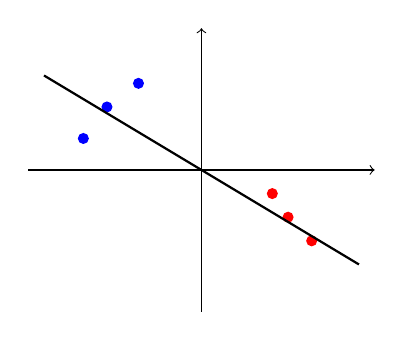
\begin{tikzpicture}
    \draw[->] (-2.2,0) -- (2.2,0);
    \draw[->] (0,-1.8) -- (0,1.8);
    \fill[blue] (-1.2,0.8) circle (2pt);
    \fill[blue] (-0.8,1.1) circle (2pt);
    \fill[blue] (-1.5,0.4) circle (2pt);
    \fill[red] (1.1,-0.6) circle (2pt);
    \fill[red] (1.4,-0.9) circle (2pt);
    \fill[red] (0.9,-0.3) circle (2pt);
    \draw[thick] (-2,1.2) -- (2,-1.2);
  \end{tikzpicture}
  \end{center}
\end{frame}

\begin{frame}{0--1 Loss}
  \[
    \ell_{0/1}(y, f(\mathbf{x})) =
    \begin{cases}
      1 & \text{if } y f(\mathbf{x}) \le 0 \\
      0 & \text{otherwise}
    \end{cases}
  \]
  \begin{itemize}
    \item Directly measures classification error.
    \item Nonconvex and non-differentiable \(\Rightarrow\) hard to optimize.
  \end{itemize}
\end{frame}

\begin{frame}{Why 0--1 Loss Is Difficult}
  \begin{itemize}
    \item Discontinuous objective with many flat regions.
    \item Gradient-based methods do not apply.
    \item Leads to combinatorial optimization.
  \end{itemize}
  \begin{block}{Idea}
    Replace with a convex, differentiable surrogate.
  \end{block}
\end{frame}

\begin{frame}{Surrogate Losses}
  Let \(z = y(\boldsymbol{w}^T \mathbf{x} + b)\).
  \begin{itemize}
    \item \textbf{Hinge loss (SVM)}:
      \[
        \ell_{\text{hinge}}(z) = \max(0, 1 - z)
      \]
    \item \textbf{Logistic loss}:
      \[
        \ell_{\text{log}}(z) = \log(1 + e^{-z})
      \]
  \end{itemize}
\end{frame}

\begin{frame}{Loss Comparison (Shape)}
  \centering
  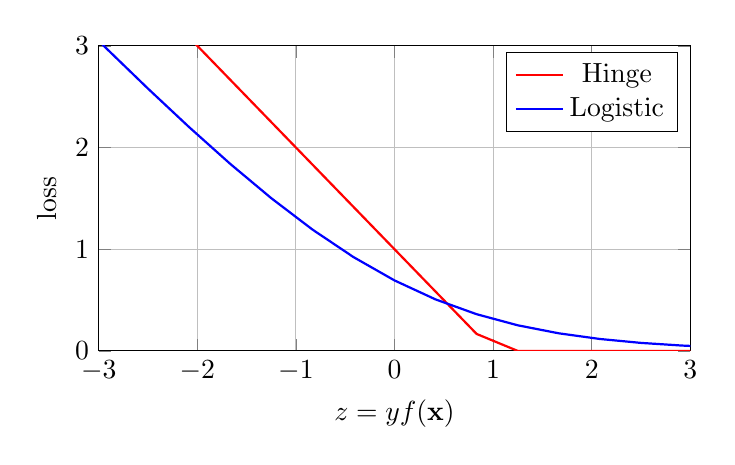
\begin{tikzpicture}
    \begin{axis}[
      width=0.75\textwidth,
      height=0.45\textwidth,
      xlabel={$z = y f(\mathbf{x})$},
      ylabel={loss},
      grid=major,
      xmin=-3, xmax=3,
      ymin=0, ymax=3
    ]
      \addplot[thick, color=red] {max(0,1-x)};
      \addlegendentry{Hinge}
      \addplot[thick, color=blue] {ln(1+exp(-x))};
      \addlegendentry{Logistic}
    \end{axis}
  \end{tikzpicture}
\end{frame}

\begin{frame}{Empirical Loss}
  Training objective (logistic example):
  \[
    \mathcal{L}(\boldsymbol{w}, b) = \frac{1}{m} \sum_{i=1}^m \log(1 + e^{-y^{(i)}(\boldsymbol{w}^T \mathbf{x}^{(i)} + b)})
  \]
  \begin{itemize}
    \item Convex in \((\boldsymbol{w}, b)\).
    \item Supports gradient-based optimization.
  \end{itemize}
\end{frame}

\begin{frame}{Regularization}
  \[
    \min_{\boldsymbol{w}, b} \; \mathcal{L}(\boldsymbol{w}, b) + \lambda \|\boldsymbol{w}\|_2^2
  \]
  \begin{itemize}
    \item Controls complexity and improves generalization.
    \item Encourages smaller weights and larger margins.
  \end{itemize}
\end{frame}

\begin{frame}{Gradient of Logistic Loss}
  For a single example with \(z = y(\boldsymbol{w}^T \mathbf{x} + b)\):
  \[
    \nabla_{\boldsymbol{w}} \ell_{\text{log}}(z)
    = -\frac{y \mathbf{x}}{1 + e^{z}}
  \]
  \[
    \frac{\partial \ell_{\text{log}}(z)}{\partial b}
    = -\frac{y}{1 + e^{z}}
  \]
  \begin{itemize}
    \item Small when correctly classified with large margin.
  \end{itemize}
\end{frame}

\begin{frame}{Gradient Descent Update}
  \[
    \boldsymbol{w} \leftarrow \boldsymbol{w} - \eta \nabla_{\boldsymbol{w}} \mathcal{L},
    \quad
    b \leftarrow b - \eta \frac{\partial \mathcal{L}}{\partial b}
  \]
  \begin{itemize}
    \item \(\eta\): learning rate.
    \item Use batch, mini-batch, or stochastic gradients.
  \end{itemize}
\end{frame}

\begin{frame}{Hinge Loss and Subgradients}
  \[
    \ell_{\text{hinge}}(z) = \max(0, 1-z)
  \]
  Subgradient:
  \[
    \partial \ell_{\text{hinge}}(z) =
    \begin{cases}
      -y\mathbf{x} & z < 1 \\
      0 & z > 1
    \end{cases}
  \]
  \begin{itemize}
    \item Use subgradient descent or SGD.
  \end{itemize}
\end{frame}

\begin{frame}{Variants of Gradient Descent}
  \begin{itemize}
    \item \textbf{Batch GD}: full dataset per update.
    \item \textbf{SGD}: one example per update.
    \item \textbf{Mini-batch}: small batch per update.
  \end{itemize}
  \begin{itemize}
    \item Trade-offs: stability vs.\ speed vs.\ variance.
  \end{itemize}
\end{frame}

\begin{frame}{Perceptron Algorithm}
  Update rule for misclassified points:
  \[
    \boldsymbol{w} \leftarrow \boldsymbol{w} + y^{(i)} \mathbf{x}^{(i)}, \quad
    b \leftarrow b + y^{(i)}
  \]
  \begin{itemize}
    \item Converges if data are linearly separable.
    \item Simple and fast, but not probabilistic.
  \end{itemize}
\end{frame}

\begin{frame}[fragile]{Logistic Regression in Python}
\begin{verbatim}
import numpy as np

def logistic_gd(X, y, eta=0.1, steps=1000):
    m, n = X.shape
    w = np.zeros(n)
    b = 0.0
    for _ in range(steps):
        scores = X @ w + b
        margins = y * scores
        probs = 1.0 / (1.0 + np.exp(margins))
        grad_w = -(1/m) * (X.T @ (y * probs))
        grad_b = -(1/m) * np.sum(y * probs)
        w -= eta * grad_w
        b -= eta * grad_b
    return w, b
\end{verbatim}
\end{frame}

\begin{frame}{Prediction and Probabilities}
  Logistic regression outputs:
  \[
    P(y=1 \mid \mathbf{x}) = \sigma(\boldsymbol{w}^T \mathbf{x} + b)
  \]
  where \(\sigma(t) = 1/(1+e^{-t})\).
  \begin{itemize}
    \item Threshold at 0.5 for class prediction.
    \item Scores can be calibrated for decision-making.
  \end{itemize}
\end{frame}

\begin{frame}{Multi-class Classification}
  \begin{itemize}
    \item Classes: \(y \in \{1,\ldots,K\}\).
    \item One-vs-rest (OvR): train \(K\) binary classifiers.
    \item Multinomial (softmax) classifier: a single model for all classes.
  \end{itemize}
\end{frame}

\begin{frame}{Softmax Model and Parameters}
  Score for class \(k\):
  \[
    s_k(\mathbf{x}) = \boldsymbol{\theta}_k^T \mathbf{x}
  \]
  Softmax probabilities:
  \[
    P(y=k \mid \mathbf{x}) =
    \frac{e^{s_k(\mathbf{x})}}{\sum_{j=1}^K e^{s_j(\mathbf{x})}}
  \]
  \begin{itemize}
    \item Parameter vectors: \(\boldsymbol{\theta}_k \in \R^n\).
    \item Parameter matrix: \(\Theta = [\boldsymbol{\theta}_1,\ldots,\boldsymbol{\theta}_K] \in \R^{n \times K}\).
  \end{itemize}
\end{frame}

\begin{frame}{Softmax Properties}
  \begin{itemize}
    \item Produces a valid probability distribution over classes.
    \item Invariant to adding a constant to all scores.
    \item Sharpness controlled by relative score differences.
  \end{itemize}
  \[
    \sum_{k=1}^K P(y=k \mid \mathbf{x}) = 1
  \]
\end{frame}

\begin{frame}{Negative Log-Likelihood (NLL)}
  For one example \((\mathbf{x}, y)\):
  \[
    \ell(\Theta; \mathbf{x}, y)
    = -\log P(y \mid \mathbf{x})
    = -\log \frac{e^{\boldsymbol{\theta}_y^T \mathbf{x}}}{\sum_{j=1}^K e^{\boldsymbol{\theta}_j^T \mathbf{x}}}
  \]
  \begin{itemize}
    \item Equivalent to cross-entropy with one-hot labels.
    \item Penalizes confident wrong predictions strongly.
  \end{itemize}
\end{frame}

\begin{frame}{Cross-Entropy Loss (Dataset)}
  One-hot label vector \(\mathbf{y}^{(i)} \in \R^K\).
  \[
    \mathcal{L}(\Theta) =
    -\frac{1}{m}\sum_{i=1}^m \sum_{k=1}^K y_k^{(i)} \log P(y=k \mid \mathbf{x}^{(i)})
  \]
  \begin{itemize}
    \item Same as average NLL.
    \item Convex in \(\Theta\) for softmax regression.
  \end{itemize}
\end{frame}

\begin{frame}{Gradient of Softmax Loss}
  Let \(P^{(i)} \in \R^K\) be predicted probabilities.
  \[
    \nabla_{\boldsymbol{\theta}_k} \mathcal{L}
    = \frac{1}{m}\sum_{i=1}^m \left(P_k^{(i)} - y_k^{(i)}\right)\mathbf{x}^{(i)}
  \]
  Matrix form:
  \[
    \nabla_{\Theta} \mathcal{L} = \frac{1}{m} X^T (P - Y)
  \]
\end{frame}

\begin{frame}{Gradient Descent Update}
  \[
    \Theta \leftarrow \Theta - \eta \nabla_{\Theta} \mathcal{L}
  \]
  \begin{itemize}
    \item Same optimization routines as binary logistic regression.
    \item Mini-batch SGD scales to large datasets.
  \end{itemize}
\end{frame}

\begin{frame}[fragile]{Softmax Regression in Python}
\begin{verbatim}
import numpy as np

def softmax(Z):
    Z = Z - Z.max(axis=1, keepdims=True)
    expZ = np.exp(Z)
    return expZ / expZ.sum(axis=1, keepdims=True)

def softmax_gd(X, Y, eta=0.1, steps=500):
    m, n = X.shape
    K = Y.shape[1]
    Theta = np.zeros((n, K))
    for _ in range(steps):
        P = softmax(X @ Theta)
        grad = (1/m) * X.T @ (P - Y)
        Theta -= eta * grad
    return Theta
\end{verbatim}
\end{frame}

\begin{frame}{Feature Engineering}
  \begin{itemize}
    \item Linear in parameters does not imply linear in inputs.
    \item Use feature maps \(\boldsymbol{\phi}(\mathbf{x})\) to capture nonlinearity.
  \end{itemize}
  \[
    \hat{y} = \text{sign}(\boldsymbol{w}^T \boldsymbol{\phi}(\mathbf{x}) + b)
  \]
\end{frame}

\begin{frame}{Common Pitfalls}
  \begin{itemize}
    \item Not scaling features (slow or unstable optimization).
    \item Using 0--1 loss directly (non-optimizable).
    \item Ignoring class imbalance (bias in predictions).
  \end{itemize}
\end{frame}

\begin{frame}{Summary}
  \begin{itemize}
    \item Linear classifiers predict via a hyperplane.
    \item 0--1 loss is replaced by convex surrogates.
    \item Gradient-based optimization scales to large data.
    \item Logistic regression yields probabilities.
  \end{itemize}
\end{frame}
